\section{Durchführung}
\label{sec:Durchführung}
Die verscheidenen Wärmeleitfähigkeiten werden mithilfe des folgenden Versuchsaufbaus
untersucht \ref{fig:aufbau}
\begin{figure}
\centering
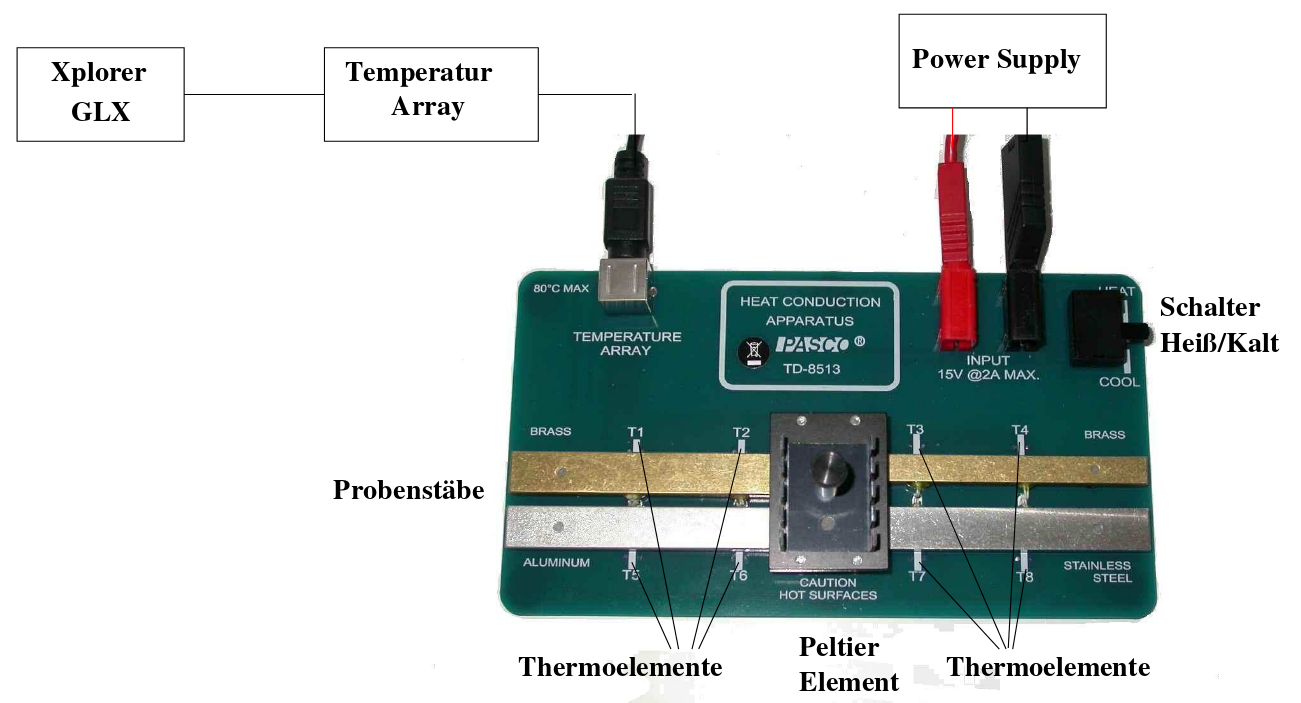
\includegraphics[width=\textwidth]{content/aufbau.png}
\caption{Versuchsaufbau.}
\label{fig:aufbau}
\end{figure}
Dabei heizt das Peltierelement die vier Metallstäbe simultan und die Temperatur wird an 8
verschiedenen Messpunkten, je zwei pro Stab, mithilfe vom Thermoelementen gemessen. Die
Messwerte werden über

\subsection{Statische Methode}
\label{sec:statische Methode}
Das Peltierelement wird mit $U_\text{P}=5V$ betrieben.
Die vier Eisenstäbe werden eine halbe Stunde lang erheitzt.
An den acht Thermoelementen wird die Temperatur gemessen und der jeweilige Wert alle 5 Sekunden gespeichert.
Anschließend werden die Stäbe durch das Peltierelement gekühlt.


\subsection{Dynamische Methode}
\label{sec:dynamische Methode}
